\chapter{Introduction} \label{ch:introduction}
Text and tables should show up.

\begin{figure}[h!]
\centering
  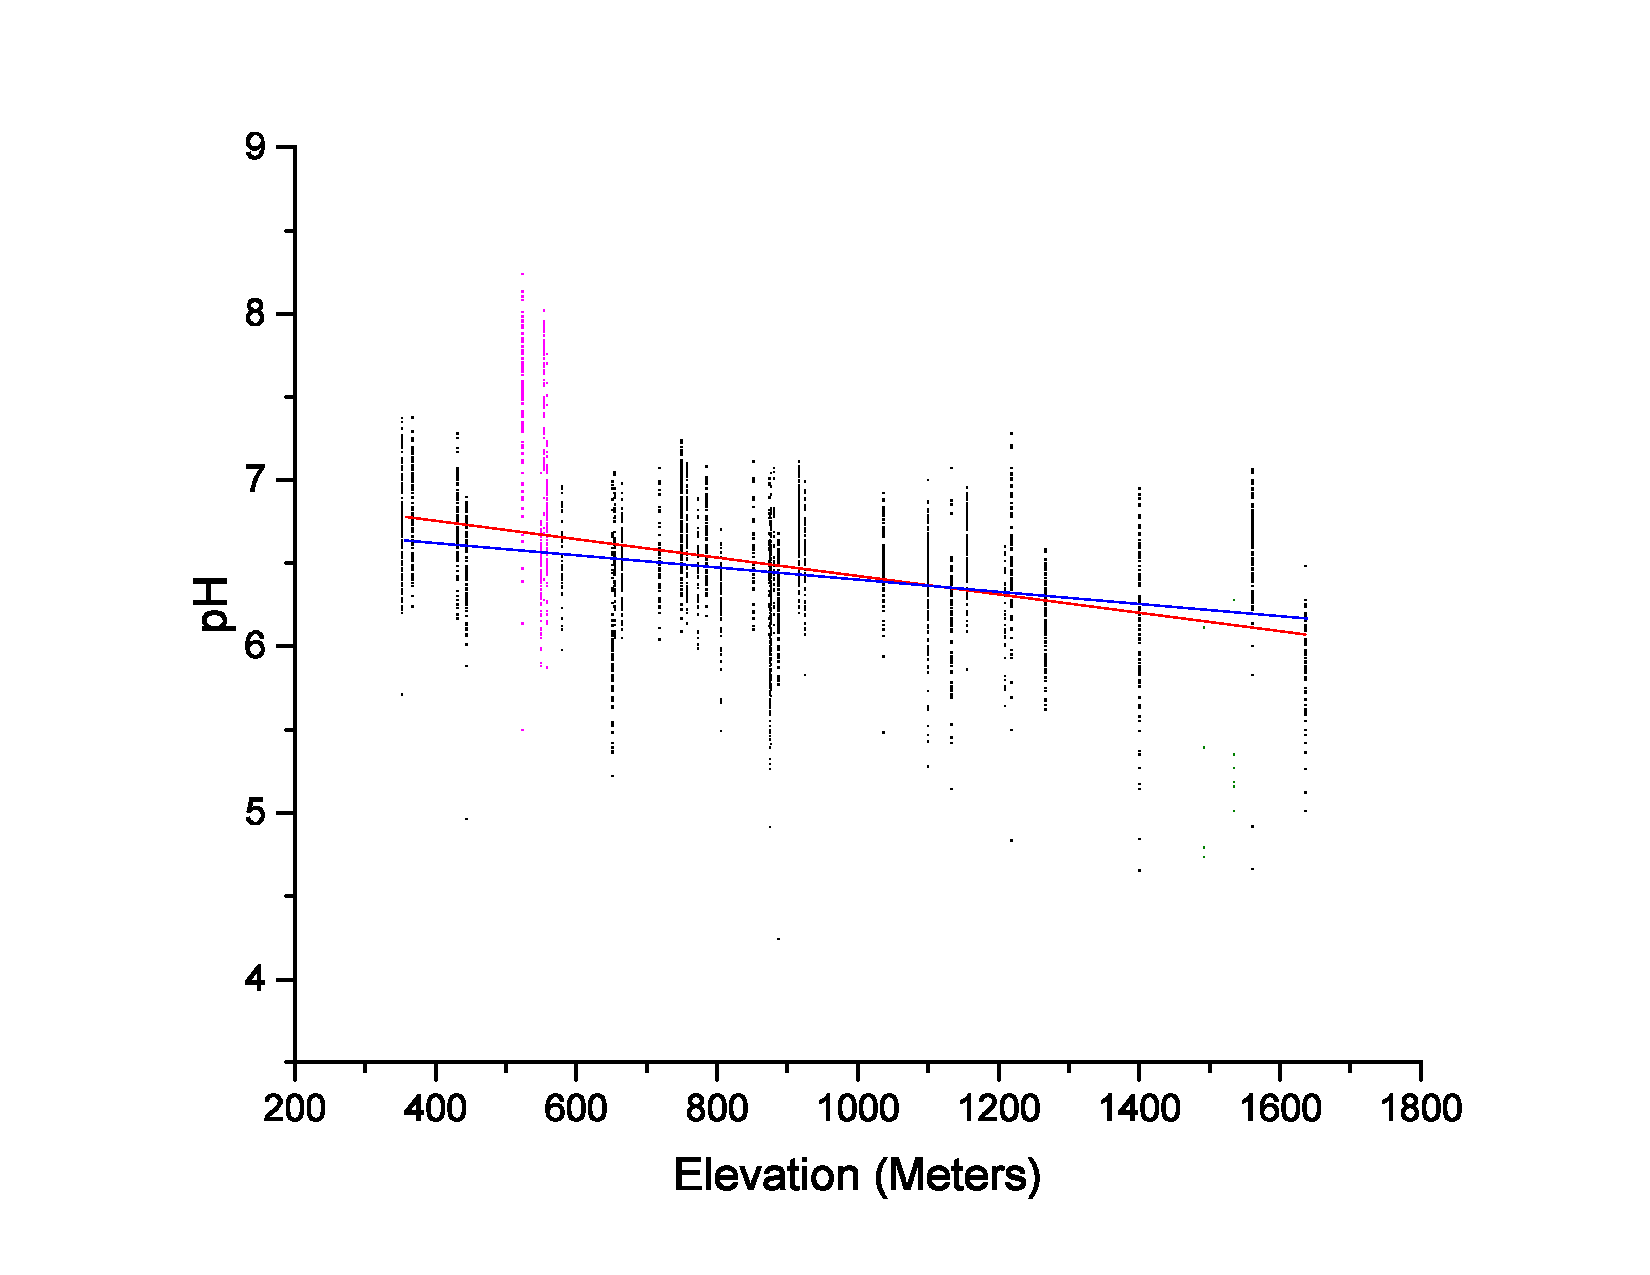
\includegraphics[width=6in]{pHdata}\\
  \caption{pH plotted vs. Elevation.  With and without outliers.}\label{fig:pHdata}
\end{figure}
\begin{verbatim}
Acid rain is believed to negatively affect The Great Smokey Mountain National Park.
Acid Deposition, more commonly known as Acid Rain, is a constant problem for the industrialized world. The amount of pollutants released into the atmosphere has risen since the industrial revolution.  The processes that industrial plants utilize excess sulfur oxides (SOx) and nitrogen oxides (NOx) into the atmosphere. This effluent production of chemicals creates problems for the world's environmental systems including acid deposition and other effects that can harm our health, our surface waters, our soils, and our structures.
Acid Deposition occurs when the emissions of sulfur oxides (SOx), and nitrogen oxides (NOx) react within the atmosphere and then the constituents and their newly created chemicals are deposited on the earth’s surface.  Acid Deposition has similar characteristics of regular precipitation but it has lower average pH of less than 4.5.  These pollutants can come down to ground in three ways: wet deposition (rain and snow), dry deposition (gases and particles), and fog or cloud deposition (occult).  Once the acid deposition constituents have entered in the environment they react with the surface waters, in the soil, and on man-made structures (Calvert, 1983).  This begins to acidify the surface waters which can harm any life forms that interact with it, it can acidify the soils and harm the plants, and it can degrade buildings.
Acid deposition greatly impacts surface water and the surrounding environment. The added pollutants affects the alkalinity of water, or its ability to buffer a change in acidity,  and results in a pH change.  As the pH level lowers, the ability of surface waters to sustain aquatic life also decline, this is called acidification. And while many factors affect the ability for the survival of aquatic life, acidification can be directly related to a lot of species survival.  
Acidification of bodies of water can be either chronic or episodic. Chronic acidification occurs when the body of water has constant low acid neutralizing capability (ANC); which creates a large area of  nearly un-inhabitable water where aquatic life would struggle to survive. Episodic acidification describes a rapid increase of acidity. Drastic acidification episodes result in large surges of nitrates and/or sulfates in surface waters. Episodes often occur during snow melts or heavy rains and are detrimental to aquatic life during the vulnerable early phases of life. (http://www.epa.gov/acidrain/effects/surface_water.html).
The Great Smoky Mountains National Park (GRSM) is located in the southern Appalachians straddling eastern Tennessee and western North Carolina.  While the second largest National Park in the eastern United States, comprising more than 220,000 hectares, it is the most-visited National Park with approximately 10 million visitors, twice the number of visitors to any other National Park, each year(Moore, 2001).  Furthermore GRSM is the largest undisturbed deciduous or coniferous forest-dominated area in the eastern United States (Delcourt and Delcourt, 1991).  The park is home to about 100 species of native trees, with the majority of the park is forest and nearly a quarter of that is old growth.  There are over 1,500 flowering plant species located in the GRSM along with 200 species of birds, 66 types of mammals, 50 native fish species, 39 kinds of reptiles, and 43 species of amphibians,  not to mention insects.  In recognition of the park's unique natural resources, the United Nations has designated GRSM as an International Biosphere Reserve, which are established to show a balance between people and nature (http://www.nps.gov/grsm/naturescience/index.htm). GRSM streams support a great number of fish species, amphibians, and benthic invertebrates; five streams in the GRSM have been designated as an Outstanding National Resource Waters (Neff, 2009).  The National Park Service (NPS) wishes to conserve the biodiversity of the park.Acid deposition negatively affects the 3,000 km of streams present in the GRSM and that impacts every living thing in the park which rely on the water quality in the park.  A literature review in (Neff 2007) approximates a pH of 6 for biological effects and a pH of 5 for mortality in trout for the park.  Exact threshold values are difficult to find because of the large number of influential factors such as species, age, egg versus fry versus adult, background water quality, exposure duration, etc.  While pH levels from 5 to 6 can be toxic in the presence of aluminum and can be harmful to eggs and fry in very soft waters in the lower end of the range.(Robinson 08).  
In order to monitor acid deposition the park has a program called the Inventory and Monitoring program.  An aspect of this program is a high elevation site, Noland Divide Watershed.  NDW is a small, 17.4 ha, watershed about 2 km east of Clingmans Dome, which is the second highest peak in the eastern US.  NDW contains sites to measure wet and dry deposition as well as "grab" samples to study in the lab.  This site is a continuation of the Integrated Forest Study (IFS) and was taken over by the park in 1991.  The IFS observed and quantified atmospheric deposition and nutrient cycling in forested watersheds.  The study demonstrated the upper elevations of the GRSM receive some of the highest loading rates of acidifying nitrogen and sulphur species in North America (Johnson and Lindberg, 1992).   The park wide Stream Survey is also part of the IFS and focuses on the park as a whole, this water quality monitoring network uses stream survey samples collected throughout the year in order to quantify water quality in the park.  Currently, samples are collected from 32 sites every two months and an additional 11 samples are collected twice per year.  These samples cover streams from 6 GRSM stream systems.  Every sample collected including NDW is processed in the lab for conductivity, pH, ANC, Chloride, Nitrate, Sulfate, Phosphate, Ammonium, Sodium, Potassium, Magnesium, Calcium, Aluminum, Copper, Iron, Manganese, Silicon, and Zinc.  Information leading to a bettering understanding of water quality conditions per watershed characteristics aids GRSM resource staff in managing the Park’s natural resources.  Other than chemistry the acidity of the park streams can be affected by geographical attributes such as geology and elevation. Stream acidification is more pronounced in higher elevation watersheds with underlying base-poor geology (Herligy et al. 1991, Hyer et al. 1995; Wigington et al. 1996a,b).  The acidification patterns along an elevational gradient occur throughout the Appalachian region similar to the data collected in the GRSM streams.  

Figure 1-1 
This figure shows all pH data from 1993 to 2012 vs. Elevation (m).  The red trend line includes abrams,  sites 237 and 252.  These outliers are removed for the blue trend line.

Figure 1 is a graph of all measured pH values for Stream Survey between the years of 1993 and 2012 graphed against the elevations they were collected.  Two notable figures are here, one that contains all pH data from 1993 to 2012 and another that has removed the outliers Abrams stream system along with sites 252 and 237.  The steeper sloped line represents the data set that still contains Abrams, sites 237, and 252.  This graph clearly illustrates pH trending downwards as elevation increases.  Increases in sulfate or nitrate in runoff and streams through acid deposition can cause an increase leaching of base cations, hydrogen ion, aluminum, and decreased ANC (Sullivan, 2004).  Leached aluminum can end up in streams and is toxic to fish (Driscoll 2003).  Rainfall and fog in the GRSM affect elevations above 4000 feet first higher elevations have steeper slopes which correlate to both thinner soils and base poor geology.  All these factors contribute to lower pH in higher elevations.  Neff et al. (2013) observed this trend, but found other basin factors correlate to chronic and episodic acidification.  Other basins factors include drainage area size, vegetation, and soil properties, which factors all are change within an elevational gradient.  
In support of GRSM natural resource management, stream water quality has been monitored since 1993, and this long-term dataset was recently statistically analyzed and commonly referred to as the “Biotic Effects Report” (Cai et al. 2013).  In this report, elevation was found to be a dominant driver for predicting water quality among the park’s stream.  Overall, results in this report found that stream pH and ANC decreased at -.32 units and -35.73 μeq L-1 respectively, per 1,000-ft elevation gain.  Conductivity, chloride, and base cations were also found to significantly decrease with elevation gain.  Sulfate showed no significant trend with elevation, however nitrate was found to significantly increase with elevation gain.  The GRSM 2011 Annual Water Quality Report compared pH trend lines representing the current 43 sites from 1993-2010 with 2011.  The data showed lines of similar slopes with different intercepts, which was interpreted to mean increasing pH at all elevations in GRSM streams.  Acid deposition increases with elevation in the GRSM and the higher elevation streams would experience increased sulfate, and prolonged acidification if soil desorption becomes a dominant geochemical watershed process which could occur if pH increased to 6.0 and sulfate dropped below 50 μeq L-1.  From a management perspective, the Biotic Effects Report contains limitations in the analyses to assess long-term changes because locations sampled have changed over time and most current sample locations are at lower elevations.

Table 1 shows the current historical elevation classes with the number of sites they include and the percent of sites in each band.  Although there were limitations, the biotic effects report provided essential information on how to improve future water quality and biological monitoring programs.
The National Park Service is currently developing a Vital Sign Monitoring Program for a number of national parks around the country, which includes the GRSM (Annual Administrative Report For Inventories and Vital Signs Monitoring FY 2010).  The goal of the GRSM Vital Sign Monitoring Program is to assess long-term changes in ecosystem health, including both terrestrial and aquatic environments. In addition, the program will integrate these environments and and include existing data on basin factors associated with water quality.   Although it is widely recognized that elevational gradient is important, a question about what elevation ranges are changing versus those that are not needs to be quantified in order to design an effective sampling program.  In addition, data must be collected at a set frequency to provide sufficient statistical power to make valid interpretations of change over time. 

Objectives of this study were to:
\begin{itemize}
\item  characterize time trends in stream pH and acidic anions among elevation ranges in order to assess whether conditions are improving or degrading, and 
\item characterize sampling variance based on available water quality data, within the context of time and elevation, to support development of the GRSM’s Vital Signs Monitoring Program.  In addition to supporting this Program, a cost analysis of selected water quality sampling schemes will be summarized.  The format of this thesis will follow these two objectives.  
\end{itemize}
\begin{itemize}
\item Has stream pH and acid anion concentrations changed among three time periods (1993-2002, 2003-2008, and 2009-2012), and among six elevation ranges (1000-2000ft, 2000-2500ft, 2500-3000ft, 3000-3500ft,3500-4500ft, 4500<)?
\begin{itemize}
 \item ANOVA
\item Time trends
\end{itemize}
\item What is the statistical power for water quality parameters based on frequency and elevational location based on historic data?
\begin{itemize}
\item Post Hoc Analysis
\item A Priori Analysis
\end{itemize}
\end{itemize}
The thesis is organized into two separate chapters following the two above research questions. Each chapter will follow the technical format of introduction, methods, results, and discussion.  
\end{verbatim}